\documentclass{article}

\usepackage{aaai}
%\usepackage{hyperref}
\usepackage{natbib}
\usepackage{amsmath}
\usepackage{graphicx}
\graphicspath{{./images/}}

\nocopyright{}
\title{Final Project: Adversarial Machine Learning in Deep Neural Networks}

\author{Brandon L.~Morris\qquad John O'Rourke\qquad Matthew Bonsall\\
  Computer Science and Software Engineering\\
  COMP 4790, Fall 2017\\
  Auburn University\\
  Auburn, AL 36832\\
  \texttt{\{blm0026, jwo0004, mvb0005\}@auburn.edu}}

\begin{document}
\maketitle


\begin{abstract}
In this project we study the topic of adversarial machine learning in the
specific context of deep artificial neural networks, commonly used in deep
learning. We specifically investigate two attacks and two defenses to a simple
convolutional neural network in the application of handwritten digit image
classification. In this way, we demonstrate both the need and effectiveness of
adversarial machine learning within deep learning.
\end{abstract}

\section{Introduction}

As we have seen throughout the semester, machine learning systems can operate
effectively under normal conditions, but can be thwarted by adversaries who
exploit characteristics of the system. For our final project we develop, attack,
defend, and analyze a machine learning system utilizing the skills cultivated
during the class. Specifically, we chose to examine adversarial machine learning
within the particular context of deep learning, where deep neural networks are
used to automatically solve a variety of complex tasks~\cite{lecun2015deep}.
We examine several attack and defenses for a convolutional neural
network~\cite{goodfellow2016deep} trained to classify images of handwritten
digits from the MNIST dataset~\cite{lecun1998mnist}.

\subsection{Deep Learning}

While it is beyond the scope of this report to provide a comprehensive overview
of deep learning, we give a brief overview to provide context of our
experimentation. Deep learning is a form of machine learning that leverages deep
artificial neural networks, trained by backpropagation~\cite{le1988theoretical}
to solve complex learning problems~\cite{goodfellow2016deep}. Many variations of
these networks exist for different categories of tasks. Since our problem domain
involves image classification, we will utilize a convolutional neural network,
since it has been shown to be extremely effective at computer vision tasks where
the data exemplifies a spatial dependency~\cite{krizhevsky2012imagenet}. Simply
put, convolutions perform perform two-dimensional dot products on overlapping
subsets of the input space with shared weights, and act as spatial feature
detectors on the input. Stacking multiple layers creates hierarchies of feature
detectors, which is similar to how the visual cortex operates in
mammals~\cite{hubel1962receptive}. A comprehensive overview of modern deep
learning can be found in~\cite{goodfellow2016deep}.

\subsection{Attacks and Defenses of Deep Neural Networks}

While deep learning has been shown to be extremely effective at tasks that were
long considered difficult for computers (such as classifying images into one of
a thousand categories~\cite{krizhevsky2012imagenet}), it too has its weakness as
a machine learning algorithm. Studies have shown that minute, expertly crafted
perturbations to otherwise correctly-handled input could lead to wildly
incorrect outputs~\cite{szegedy2013intriguing}. This malicious inputs are
typically known as \textit{adversarial examples}, and are consistently found
within deep learning. An sample of an adversarial example can be seen in
Figure~\ref{fig:ax-example}. Even machine learning algorithms that do not utilize deep
neural networks are susceptible to adversarial
examples~\cite{papernot2016transferability}.

\begin{figure}
  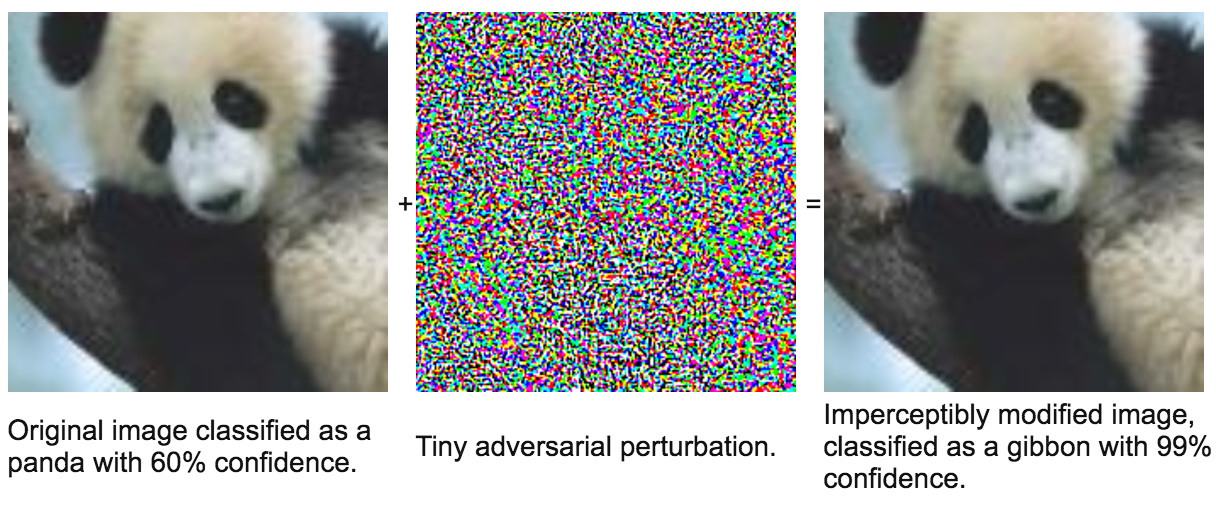
\includegraphics[width=0.5\textwidth]{ax-example}
  \caption{An adversarial example. Left: A normal input to the classifier,
  correctly classified as a panda with 60\% confidence. Center: The adversarial
perturbation, to be combined with the original input and constrained to have
minimal impact. Right: The adversarial example. While imperceptibly different
than the original image on the left, the deep neural network misclassifies this
image with high confidence.}
\label{fig:ax-example}
\end{figure}

There are numerous ways to craft adversarial
examples~\cite{szegedy2013intriguing,goodfellow2014explaining,nguyen2015deep,papernot2016limitations,carlini2017towards},
we will only experiment with two such attacks. Both of these attacks are
described in greater detail in the next section, and both rely on the
\textit{gradient} of the neural network (which is essential during training) to
exploit the classifier by finding minute perturbations that create a maximal
different in the output.

As demonstrated in our experiments (Experiments section), both of these
attacks have a severe impact on the performance of our otherwise performant
classifier. To combat the adversary employing these attacks, we utilize two
defenses in an attempt to increase the model's accuracy to the malicious inputs.
Both of these strategies are discussed in the next section.

\section{Methodology}

We now describe our approach to attacking and defending a deep neural network
classifier. Our classification problem involves classifying handwritten digits
from the MNIST data set~\cite{lecun1998mnist}. Figure~\ref{fig:mnist-example}
portrays the kind of images our classifier handles as input. All the code
utilized to carry out these was developed in Python. We utilized the TensorFlow
machine learning library~\cite{abadi2016tensorflow} for accelerated computation
and the Keras library~\cite{chollet2015keras} to facilitate development. To
generate adversarial examples, we utilized standard implementations in the
Cleverhans library~\cite{goodfellow2016cleverhans} to ensure correctness.

\begin{figure}
  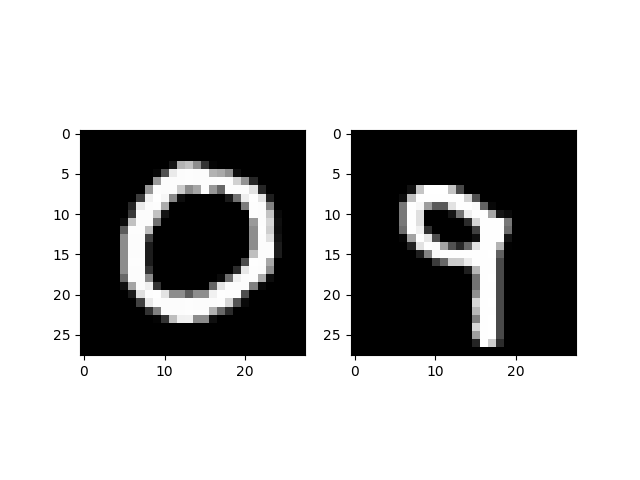
\includegraphics[width=0.5\textwidth]{normal}
  \caption{Two test images from the MNIST data set. The raw pixel values are the
  inputs to the classifier, which attempts to output the digit the image
represents (e.g\@. 0 for the left image and 9 for the right image).}%
  \label{fig:mnist-example}
\end{figure}

\subsection{Attack 1: Fast Gradient Sign Method}

The Fast Gradient Sign Method (FGSM) was first introduced
in~\cite{goodfellow2014explaining} and has since become a very popular choice
for attacking deep learning models given its computational ease and
effectiveness. FGSM relies only on the gradient of the network with respect to
its input, and can be computed in one backpropagation pass. Specifically, FGSM
utilizes the \textit{sign} of the input gradient, then perturbs the input in
that direction by a small amount $\epsilon$. In equation form, the adversarial
example is computed as

\begin{equation}
  x^* = x + \epsilon \cdot {\text{sign}}(\nabla_xJ_\theta(x, y))
\end{equation}

\noindent
Where $x$ is the input being perturbed, $J$ is the cost function of the network,
and $y$ is the true label. The result is that the input is modified such that it
minimizes the confidence in the correct label, and the modification is
imperceptibly small provided $\epsilon$ is sufficiently small. Note that FGSM
will modify most or all of the image, but each modification will be very small.
Some examples of adversarial examples crafted via the FGSM algorithm can be seen
in Figure~\ref{fig:fgsm-ax}.

\begin{figure}
  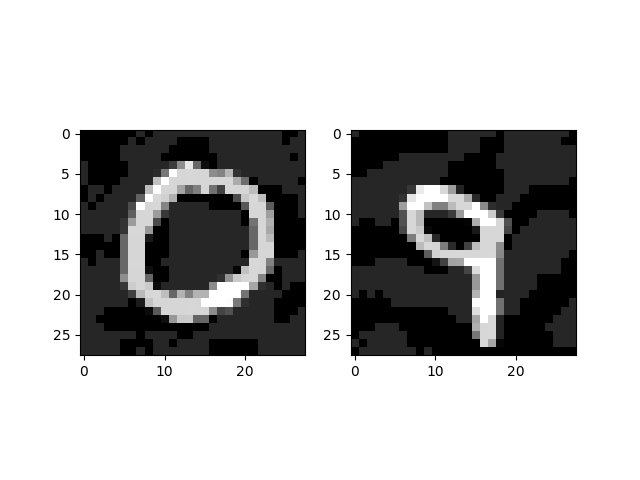
\includegraphics[width=0.5\textwidth]{fgsm}
  \caption{Two images of adversarial inputs crafted by the FGSM
    algorithm~\cite{goodfellow2014explaining}. Note
  that almost all of the pixels have been modified, but only slightly (here
$\epsilon = 0.15$). While the digit in inside the image is still plainly obvious
to human inspection, the performant deep learning classifier often incorrectly
classifies this kinds of images.}%
  \label{fig:fgsm-ax}
\end{figure}

\subsection{Attack 2: Jacobian Saliency Map Algorithm}

The second attack we utilize is called the Jacobian Saliency Math Algorithm
(JSMA), and was first introduced in~\cite{papernot2016limitations}. Similar to
FGSM, the JSMA algorithm utilizes the gradient of the network with respect to
the input to calculate perturbations. However, JSMA utilizes a ``forward
derivative'' of the network itself (rather than the cost function), which is
also known as the Jacobian. Utilizing the Jacobian, JSMA creates a
\textit{saliency map} that graphs how sensitive the model's output its to
particular features in the input space. It then selects pairs of pixels to
modify until the image is sufficiently adversarial, or the maximum number of
features have been modified. In our experiments, we limited the number of pixels
that could be modified to 10\% of the input space, in order to maintain
sufficiently small perturbations. Figure~\ref{fig:jsma-ax} demonstrates what
images that have been modified by JSMA look like.

\begin{figure}
  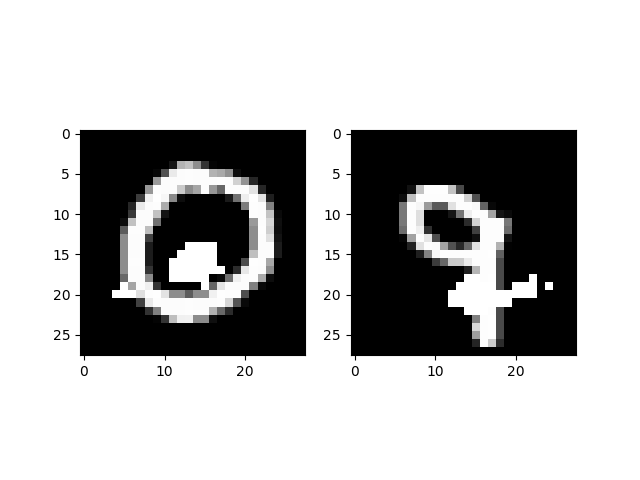
\includegraphics[width=0.5\textwidth]{jsma}
  \caption{Two images of adversarial inputs crafted by the JSMA
    algorithm~\cite{papernot2016limitations}. While only a few pixels were
  modified, it is easy to tell that they have been modified drastically.}%
  \label{fig:jsma-ax}
\end{figure}

\subsection{Defense 1: Adversarial Training}

The first defensive strategy we investigate for this project is known as
\textit{adversarial training}~\cite{goodfellow2014explaining}. This defense
involves crafting adversarial examples, then incorporating those new inputs into
the dataset. The idea is that adversarial examples exist outside the
distribution of normal inputs, so a model only trained on normal inputs will
have great difficulty properly handling adversarial examples. By augmenting the
data set to include adversarial inputs, the model has a chance of appropriately
handling them, since it has seen data from that distribution before.

The basic algorithm we utilized goes as follows:
\begin{enumerate}
  \item Train a classifier on normal inputs
  \item Generate adversarial examples on the training data by either FGSM or JSMA
  \item Train a \textit{new classifier} on both the normal and adversarial
    training inputs
\end{enumerate}
The new classifier resulting from adversarial training is then evaluated under
normal inputs and adversarial examples.

\subsection{Defense 2: Denoising Autoencoder}

Our second defensive strategy attempts to scrub the adversarial perturbations
from inputs before they are classified by the neural network, as a preprocessing
step. To do this, we make use of a denoising autoencoder (DAE). Autoencoders are
commonly used in deep learning, and are neural networks that learn to map inputs
back to themself, usually with some additional
constraint~\cite{goodfellow2016deep}. Since these neural networks usually
involve layers that shrink to a smaller latent space (i.e\@. encoding) and then
growing back to the original input space (i.e\@. decoding), they can be thought
of as automatically learning a coding coding scheme for the input. In our case,
a denoising autoencoder performs this process utilizing noisy inputs to start
and mapping them to the original clean inputs.

Since most adversarial perturbations are small (see
Figures~\ref{fig:ax-example},~\ref{fig:fgsm-ax}, and~\ref{fig:jsma-ax}), it
stands to reason that a preprocessing step that removes noise might also remove
adversarial perturbations. While this type of preprocessing has been explored
before in the literature~\cite{graese2016assessing,shenape}, we could not find
another example that explicitly used denoising autoencoders in this way.

\section{Experiments}

\section{Results}

% Baseline:       97.39
% FGSM:           42.47
% JSMA:           4.37
% AX TRAINING
% FGSM: Normal    98.45
% FGSM: AX        98.25
% JSMA: Normal    98.58
% JSMA: AX orig   95.95
% JSMA: AX new    4.36
% DAE
% Normal+DAE      96.95
% FGSM+DAE        89.33
% FGSM+JSMA       63.42

\section{Breakdown of Work}

%\bibliographystyle{aaai}
\bibliographystyle{plain}
\bibliography{references}

\end{document}
